\chapter{EXPERIMENTS AND RESULTS}
	\label{CH_05}
\section{Data}
In this project, two public available datasets are used, CB6133 produced with PISCES CullPDB\cite{wang2003pisces} and CB513. To better evaluate the performance of the network, a smaller filtered version of CB6133 is formed by removing redundant sequences in CB6133 that have over 25\% similarity with some sequence in CB513. 80\% of the filtered CB6133 dataset are random selected as training set and the rest are the validation set. CB513 here is the standard test set.
Both CB513 and filtered CB6133 can be found at http://www.princeton.edu/~jzthree/datasets/ICML2014/.
\section{Experiments}
In the following experiments, all network structures are trained using the pipeline described in Chapter \ref{CH_04}. The system calculate the validation performance every 50 iterations(batch). The early stop strategy is based on the valid accuracy, if the system doesn't get better accuracy for 30 times of validation it stops training. That approximates to a tolerance of 23 epochs. And the best model get from training will be evaluated using CB513. 
All the experiment are run on an Alienware desktop with Intel core i7-4700MQ CPG @ 2.4GHz×8, 23.5 GB memory and Geforce GTX 780M GPU.

\subsection{Experiment on loss function}
To demonstrate the effectiveness of the modified loss function described in chapter \ref{CH_04}, comparison is made between the test result of several different architectures with regular loss and modified loss function. All the architectures been tested and the results are listed in Table \ref{tb:exp_loss}. The first four columns are models without RNN layer, with 1, 2 and 3 RNN layers respectively. They are trained with regular loss function. The other fours are the same models which been trained with modified loss functions. As you can see in Figure \ref{fig:exp_loss}, all the model with modified loss function(red bars) achieved higher test accuracy than models with regular loss function(blue bar). Which means the modified loss function performs better when the input data has variable length. So in other experiments, only modified loss function are used.\par 
\begin{table}[h] \label{tb:exp_loss}
	\centering
	\begin{tabular}{llllr}
	\hline
	\multicolumn{4}{c}{Model} &
	\multicolumn{1}{c}{Performance}\\
	\cline{1-4}
	Multi conv & RNN  & Output layers &  loss & test accuracy(\%)\\
	\hline
	64 channels & - & fc &regular &63.1\\
	64 channels & \begin{tabular}{@{}c@{}}1 layer \\ static 50\end{tabular} & fc &regular &63.1\\
	64 channels & \begin{tabular}{@{}c@{}}2 layer \\ static 50\end{tabular} & fc &regular &65.7\\
    64 channels & \begin{tabular}{@{}c@{}}3 layer \\ static 50\end{tabular} & fc &regular &66.2\\
    \cline{1-5}
    64 channels & - & fc &modified &63.5\\
	64 channels & \begin{tabular}{@{}c@{}}1 layer \\ static 50\end{tabular} & fc &modified &68.0\\
	64 channels & \begin{tabular}{@{}c@{}}2 layer \\ static 50\end{tabular} & fc &modified &68.0\\
    64 channels & \begin{tabular}{@{}c@{}}3 layer \\ static 50\end{tabular} & fc &modified &67.8\\
	\hline
	\end{tabular}
	\caption[result of different loss functions]{result of different loss functions}
\end{table}

\begin{figure}[H] 
	\centering
	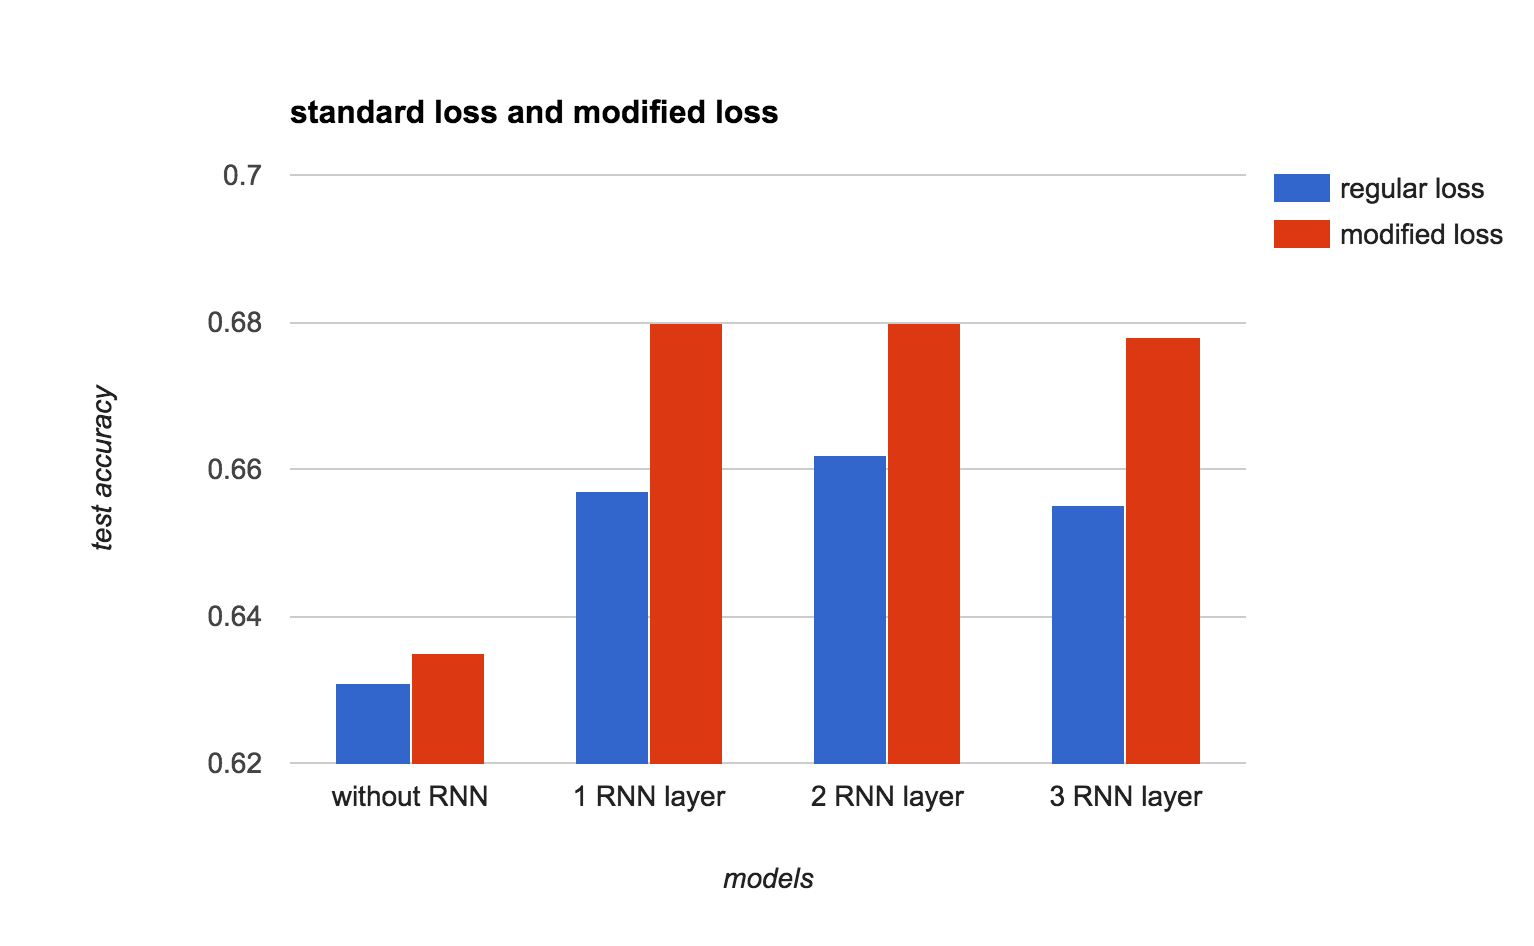
\includegraphics[width=6in]{Figures/exp_loss}
	\caption[result of different loss functions]{result of different loss functions}
	\label{fig:exp_loss}
\end{figure}

\subsection{Experiment of different output layers}
This experiment compares the performance of models using fully connected layers and convolutional layers at the end of the network, as described in section \ref{sec:output_layer}. As listed in Table \ref{tb:exp_output_layer}, the first three models use fully connected layers as output layers. The other three are the same model replacing the fully connected layers with convolutional layers. The first kernel size is 3 and the second kernel size is 11. As illustrate in Figure \ref{fig:exp_fc_conv} the convolutional layers improve the performance of all three models by at least 1 percent. The difference between fully connected a layer and a convolutional layer here is the kernel size. The fully connected layer in this project is equivalent to a convolutional layer with kernel size 1. So this means that when the network making final prediction of secondary structures, considering more context information is helpful. In addition, this kind of context information can not be fully captured by the previous RNN layers.
\begin{table}[h] \label{tb:exp_output_layer}
	\centering
	\begin{tabular}{llcr}
	\hline
	\multicolumn{3}{c}{Model} &
	\multicolumn{1}{c}{Performance}\\
	\cline{1-3}
	Multi conv & RNN  & Output layers & test accuracy(\%)\\
	\hline
	64 channels & - & fc  &63.1\\
	64 channels & \begin{tabular}{@{}c@{}}1 layer \\ dynamic 128\end{tabular} & fc  &68.13\\
    64 channels & \begin{tabular}{@{}c@{}}2 layer \\ dynamic 128\end{tabular} & fc  &68.02\\
    \cline{1-4}
    64 channels & - & conv &65.4\\
	64 channels & \begin{tabular}{@{}c@{}}1 layer \\ dynamic 128\end{tabular} & conv &69.2\\
    64 channels & \begin{tabular}{@{}c@{}}2 layer \\ dynamic 128\end{tabular} & conv &69.5\\
	\hline
	\end{tabular}
	\caption[result of different output layers]{result of different output layers}
\end{table}

\begin{figure}[H] 
	\centering
	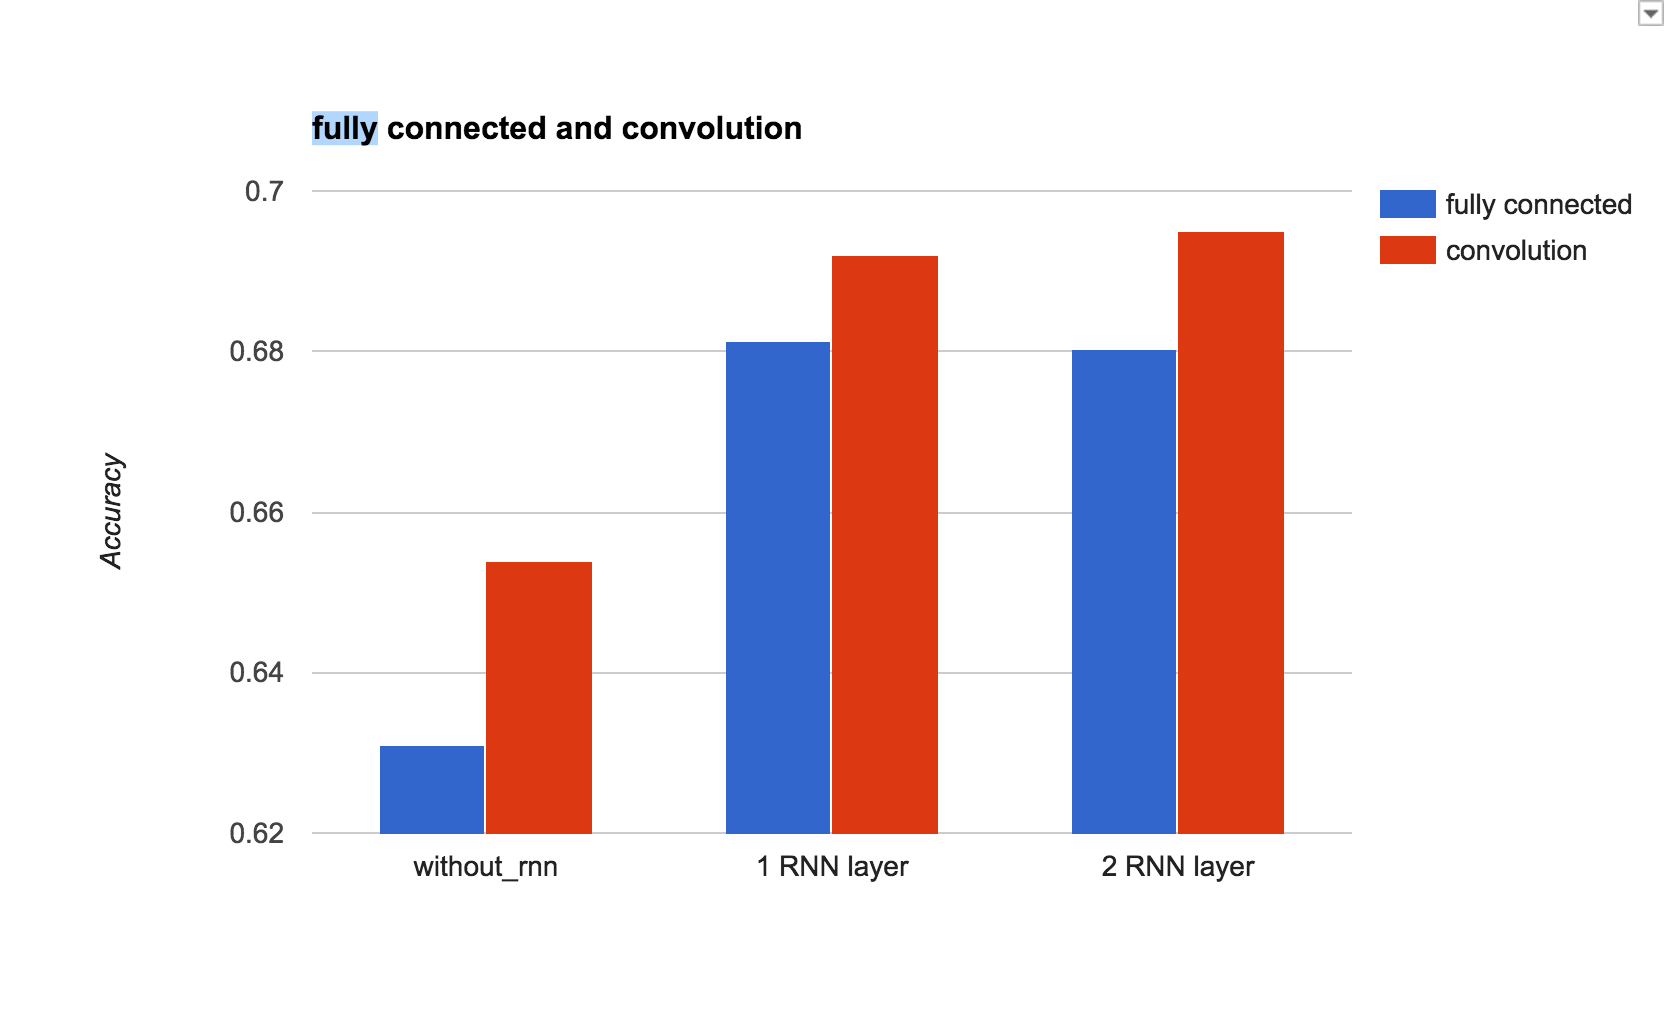
\includegraphics[width=6in]{Figures/exp_fc_conv}
	\caption[result of different output layers]{result of different output layers}
	\label{fig:exp_fc_conv}
\end{figure}

\subsection{Experiment of different hidden unit in RNN layer}
This experiment focuses on how does the hidden unit number in RNN layer affect the performance of the model. Only 1 layer bidirectional RNN are used here because a series of model need to be tested and using more than 1 layer of RNN the experiment would take too long. As shown in table \ref{tb:exp_rnn_unit}, a model without RNN layer are the baseline, then four models with 2, 10, 32 and 128 hidden units RNN layer have been evaluated. Figure \ref{fig:exp_hidden} is the line chart of accuracy vs hidden unit number. As you can see, with a very small number of 2 hidden units 1 RNN layer can improve the accuracy by 2\%. From 2 to 30 units it improve the accuracy by 0.8\%, and from 30 to 128 the improvement is only 0.5\%.  
\begin{table}[H] \label{tb:exp_rnn_unit}
	\centering
	\begin{tabular}{llcr}
	\hline
	\multicolumn{3}{c}{Model} &
	\multicolumn{1}{c}{Performance}\\
	\cline{1-3}
	Multi conv & RNN  & Output layers & test accuracy(\%)\\
	\hline
	64 channels & - & conv &65.4\\
	64 channels & \begin{tabular}{@{}c@{}}1 layer \\ dynamic 2\end{tabular} & conv  &67.9\\
	64 channels & \begin{tabular}{@{}c@{}}1 layer \\ dynamic 10\end{tabular} & conv  &68.2\\
	64 channels & \begin{tabular}{@{}c@{}}1 layer \\ dynamic 32\end{tabular} & conv  &68.7\\
	64 channels & \begin{tabular}{@{}c@{}}1 layer \\ dynamic 64\end{tabular} & conv  &68.8\\
	64 channels & \begin{tabular}{@{}c@{}}1 layer \\ dynamic 128\end{tabular} & conv  &69.2\\
	\hline
	\end{tabular}
	\caption[result of different hidden unit numbers]{result of different hidden unit numbers}
\end{table}
To further demonstrate the performance on individual secondary structures, a precision vs number of unit graph is ploted in Figure \ref{fig:exp_hidden_detail}. The y axis is the precision for each class of secondary structure, the x axis is the number of units in RNN layer, zero represent without RNN layer. The number after the label in legend is the frequencies of these secondary structures appear in protein structures. As shown, basically the higher the frequency is, the higher the precision is. The model without the RNN layer can achieve comparable precision on the high frequency secondary structures. However it fails to predict class B, G and I. The RNN layer, even with very few hidden units, significantly improves the performance on low frequency classes. While the number of hidden units increase, the model tend to have higher precision on those rare classes. However the model still fail to predict the class I which is super rare in training dataset. \par
\begin{figure}[h] 
	\centering
	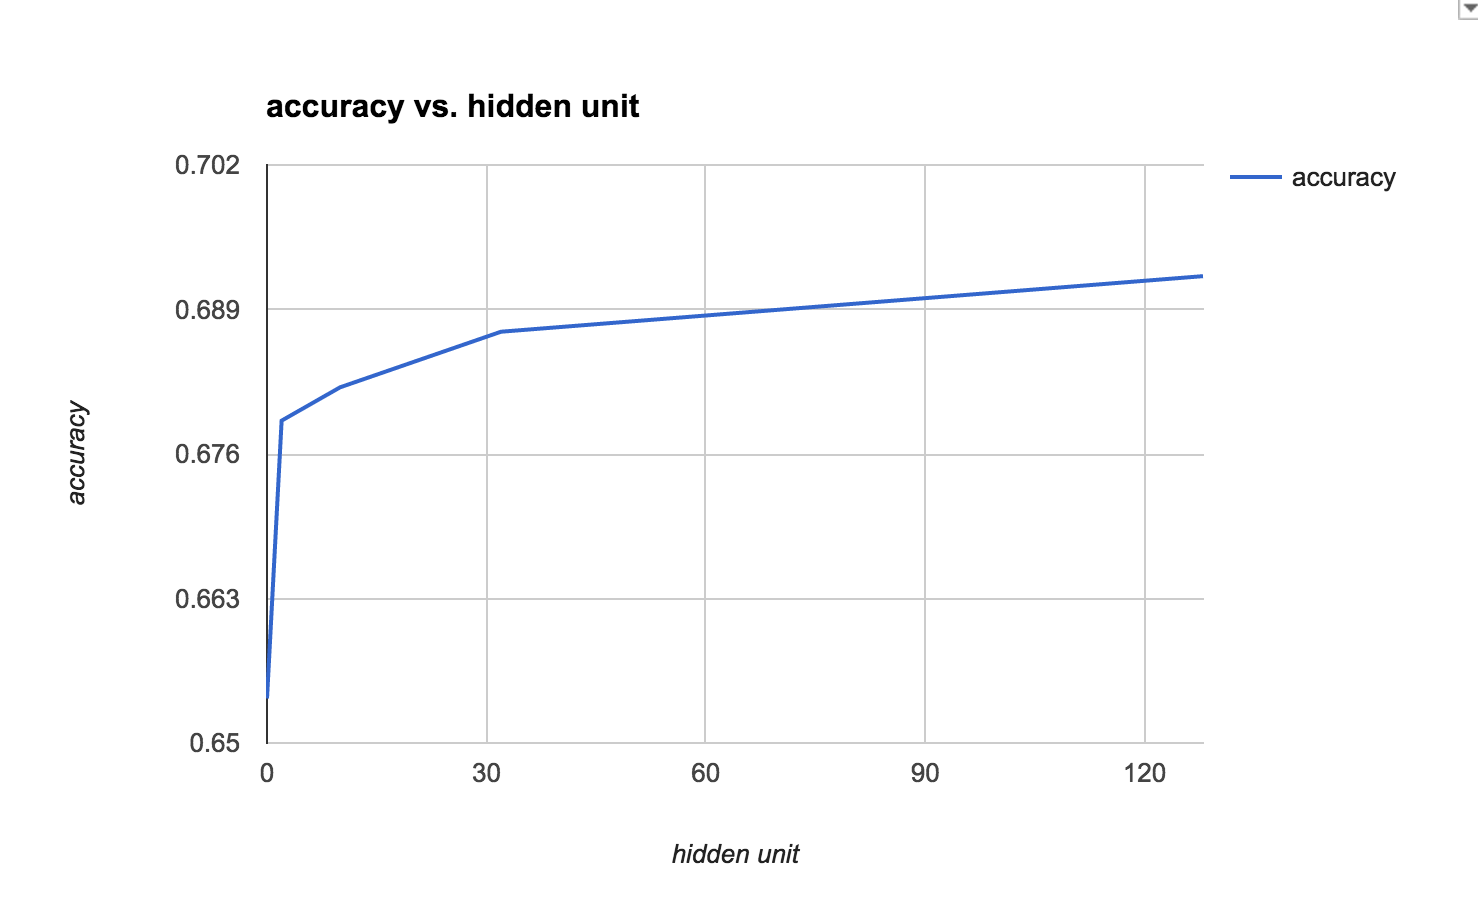
\includegraphics[width=6in]{Figures/exp_hidden}
	\caption[result of different hidden unit numbers]{result of different hidden unit numbers}
	\label{fig:exp_hidden}
\end{figure}

\begin{figure}[h] 
	\centering
	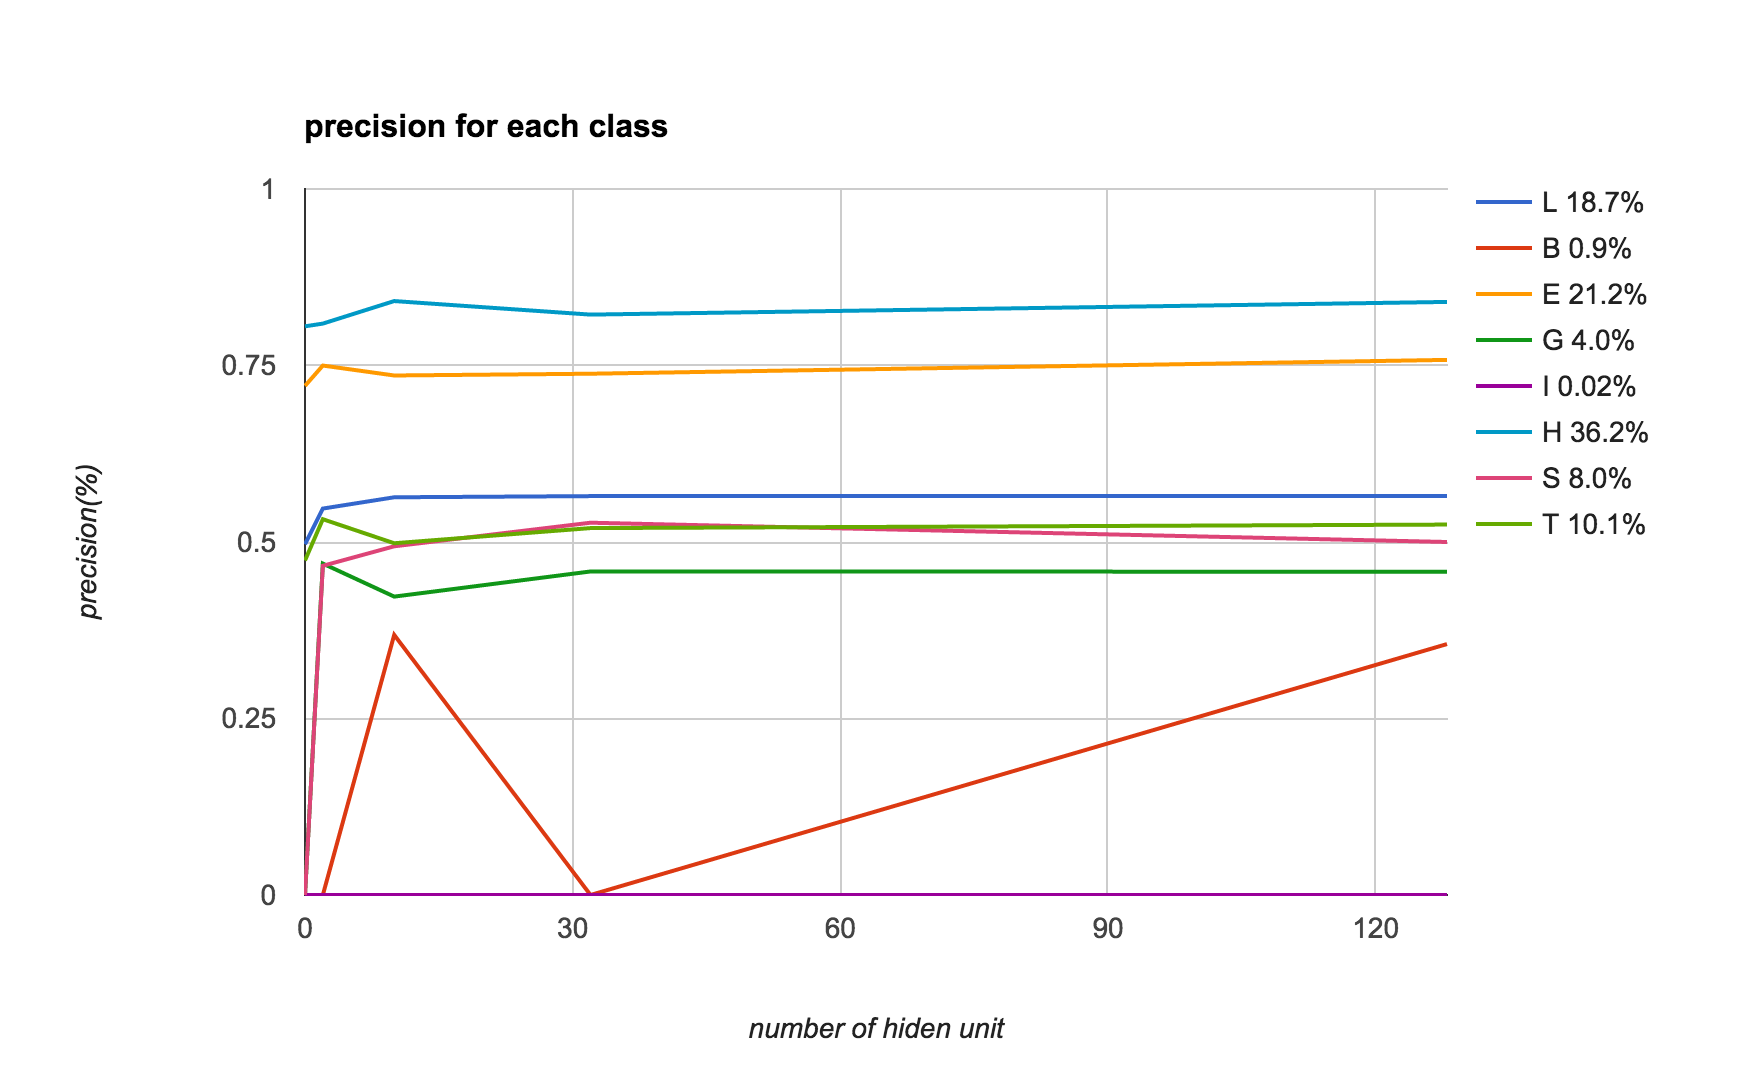
\includegraphics[width=6in]{Figures/exp_hidden_detail}
	\caption[Detail result of different hidden unit numbers]{Detail result of different hidden unit numbers}
	\label{fig:exp_hidden_detail}
\end{figure}

\subsection{Final result}
The best model from all these experiments in previous sections is the model with 2 layers of 128 hidden units bidirectional RNN with convolutional output layer. The test accuracy on CB513 is 69.5\%. To train this model, it took about 20 hours on the computer described at the beginning of this Chapter. \par

